\documentclass[tikz,border=6pt]{standalone}
\usepackage{pgfplots}
\pgfplotsset{compat=1.18}
\usepgfplotslibrary{colormaps}
\usetikzlibrary{arrows, arrows.meta, calc}
\usetikzlibrary{decorations.markings}


\usepackage{amssymb,amsmath,mathtools}

\usepackage[T1]{fontenc}
\usepackage[utf8]{inputenc}
\usepackage{newpxtext,newpxmath}
\usepackage{sectsty}

\renewcommand{\Re}{\operatorname{\mathrm{Re}}}
\renewcommand{\Im}{\operatorname{\mathrm{Im}}}

\begin{document}
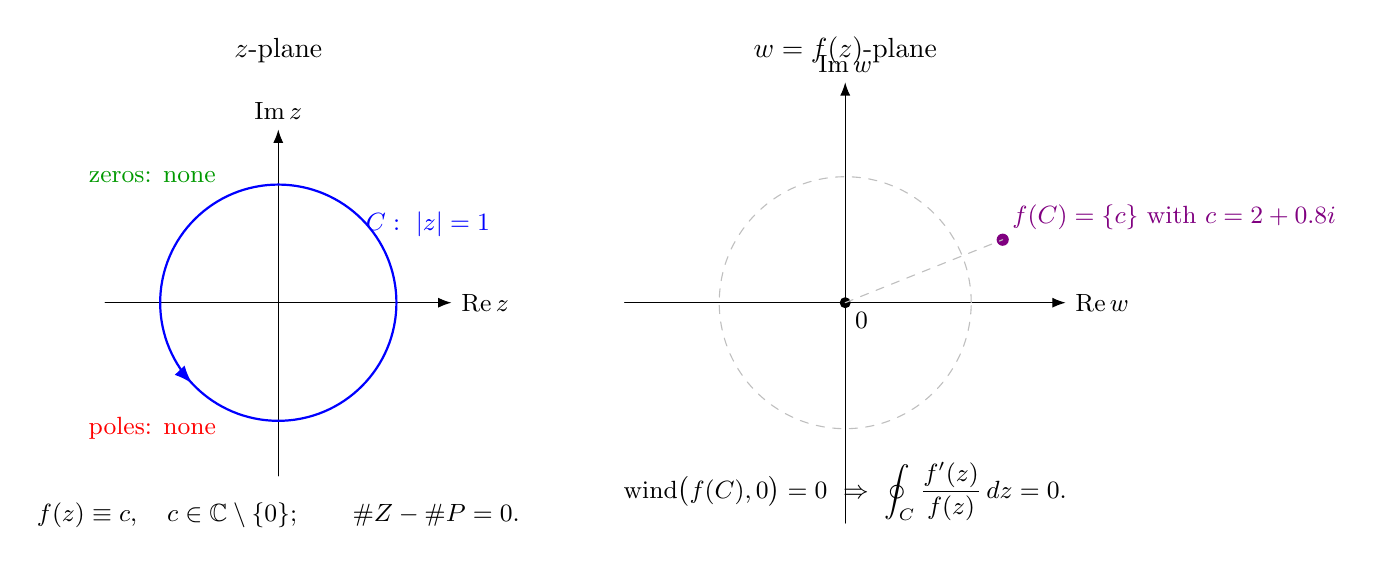
\begin{tikzpicture}[>=Latex, line cap=round, line join=round, font=\small]

% ================= Left: z-plane =================
\begin{scope}
	\node[font=\normalsize] at (0,3.2) {$z$-plane};
	\draw[->] (-2.2,0)--(2.2,0) node[right] {$\Re z$};
	\draw[->] (0,-2.2)--(0,2.2) node[above] {$\Im z$};
	
	% C: unit circle (positively oriented)
	\draw[blue,thick,postaction={decorate},
	decoration={markings, mark=at position 0.62 with {\arrow{>}}}]
	(0,0) circle (1.5);
	\node[blue] at (1.9,1.0) {$C:\ |z|=1$};
	
	% No zeros/poles inside
	\node[green!60!black] at (-1.6,1.6) {zeros: none};
	\node[red] at (-1.6,-1.6) {poles: none};
	
	% Function label
	\node[align=left] at (0,-2.7) {$\displaystyle
		f(z)\equiv c,\quad c\in\mathbb{C}\setminus\{0\};\qquad
		\#Z-\#P=0.$};
\end{scope}

% =============== Right: w-plane ==================
\begin{scope}[shift={(7.2,0)}]
	\node[font=\normalsize] at (0,3.2) {$w=f(z)$-plane};
	\draw[->] (-2.8,0)--(2.8,0) node[right] {$\Re w$};
	\draw[->] (0,-2.8)--(0,2.8) node[above] {$\Im w$};
	
	% origin
	\fill (0,0) circle(2pt) node[below right] {$0$};
	
	% choose a concrete constant c = 2 + 0.8 i
	\coordinate (C) at (2.0,0.8);
	
	% image of C is the single point c
	\fill[violet] (C) circle (2.2pt);
	\node[violet,above right] at (C) {$f(C)=\{c\}$ with $c=2+0.8i$};
	
	% faint dashed circle around c just to suggest “no winding around 0”
	\draw[gray!50,dashed] (0,0) circle (1.6); % purely illustrative backdrop
	\draw[gray!50,dashed] (0,0) -- (C);
	
	% annotation
	\node[align=center] at (0,-2.4)
	{$\mathrm{wind}\big(f(C),0\big)=0
		\ \Rightarrow\ 
		\displaystyle \oint_C \frac{f'(z)}{f(z)}\,dz=0.$};
\end{scope}

\end{tikzpicture}
\end{document}
